% ===========================================================================
\chapter{Introdu\c{c}\~ao}
% ===========================================================================

\section{Contextualiza\c{c}\~ao}

A modelagem tridimensional \'e, na engenharia contempor\^anea, uma atividade de projeto e n\~ao
apenas de ilustra\c{c}\~ao. Um modelo de superf\'icie de um ve\'iculo automotivo codifica
decis\~oes geom\'etricas --- curvaturas, tangentes, dimens\~oes de envelope, folgas --- que podem
ser verificadas, medidas e reproduzidas. Quando esse modelo nasce de um processo manual e
interativo, por\'em, boa parte dessas decis\~oes permanece impl\'icita: vive na mem\'oria de
quem operou o \emph{software}, e n\~ao em um artefato audit\'avel. \'E comum que um ajuste de
malha bem-sucedido n\~ao possa ser reconstru\'ido depois, porque foi feito com o mouse, em uma
sequ\^encia de gestos que ningu\'em registrou \cite{bbotsch2010}.

Em paralelo, os protocolos de integra\c{c}\~ao entre modelos de linguagem de grande porte e
ferramentas externas amadureceram rapidamente. O \emph{Model Context Protocol} (MCP)
\cite{mcpspec2024} prop\~oe uma interface padronizada, baseada em mensagens JSON-RPC~2.0
\cite{jsonrpc2020}, para que um agente de intelig\^encia artificial descubra e invoque
ferramentas expostas por um servidor. Um servidor MCP para o Blender permite que um agente
execute c\'odigo Python na sess\~ao viva do programa, inspecione a cena e capture imagens da
\emph{viewport}. Isso desloca a unidade de trabalho: deixa de ser o gesto e passa a ser o
\emph{script}, que \'e version\'avel, revis\'avel e reproduz\'ivel.

A conflu\^encia desses dois movimentos --- formaliza\c{c}\~ao da geometria e automa\c{c}\~ao por
agentes --- abre a possibilidade de tratar a modelagem de um ve\'iculo como um problema de
engenharia de software: com requisitos identificados, decis\~oes de arquitetura registradas,
crit\'erios de aceita\c{c}\~ao observ\'aveis e evid\^encia de verifica\c{c}\~ao rastre\'avel.

\section{Problema de pesquisa}

O problema que orienta este trabalho pode ser enunciado da seguinte forma:

\begin{quote}
\emph{\'E poss\'ivel produzir, de forma integralmente reprodut\'ivel e automatizada por um
agente de intelig\^encia artificial por meio do Model Context Protocol, um modelo tridimensional
de um autom\'ovel esportivo cuja geometria e materiais sejam fi\'eis a refer\^encias fotogr\'aficas
dispon\'iveis, atendendo simultaneamente a restri\c{c}\~oes de topologia de malha adequada \`a
subdivis\~ao e a um envelope dimensional verificado?}
\end{quote}

Do enunciado derivam tr\^es tens\~oes t\'ecnicas que precisam ser resolvidas conjuntamente. A
primeira \'e a \textbf{tens\~ao entre fidelidade e automa\c{c}\~ao}: refer\^encias fotogr\'aficas
s\~ao perspectivas, com distor\c{c}\~ao e oclus\~ao, e n\~ao blueprints ortogr\'aficos; converter
fotografias em par\^ametros geom\'etricos exige um m\'etodo expl\'icito de estimativa. A segunda
\'e a \textbf{tens\~ao entre expressividade e restri\c{c}\~ao topol\'ogica}: reproduzir recortes,
arcos de roda e entradas de ar em geral se faz com opera\c{c}\~oes booleanas, que produzem
n-gons e tri\'angulos em arestas vis\'iveis, incompat\'iveis com subdivis\~ao de qualidade. A
terceira \'e a \textbf{tens\~ao entre realismo f\'isico e custo computacional}: pintura
automotiva convincente requer \emph{clear coat}, micro-flocos met\'alicos e transmiss\~ao em
vidros, o que demanda um modelo de sombreamento fisicamente plaus\'ivel
\cite{burley2012, karis2013}.

\section{Hip\'otese}

A hip\'otese de trabalho \'e que a combina\c{c}\~ao de tr\^es elementos --- (i) uma
especifica\c{c}\~ao formal com requisitos e crit\'erios de aceita\c{c}\~ao observ\'aveis,
(ii) gera\c{c}\~ao de geometria exclusivamente por c\'odigo determin\'istico, com as
restri\c{c}\~oes topol\'ogicas impostas no n\'ivel do algoritmo, e (iii) media\c{c}\~ao de todas
as opera\c{c}\~oes destrutivas por um agente conectado via MCP --- permite obter um modelo cuja
ader\^encia \`a refer\^encia \'e compar\'avel \`a de um fluxo manual equivalente, mas cuja
reprodutibilidade e auditabilidade s\~ao substancialmente superiores.

\section{Justificativa}

A justificativa do trabalho se apoia em tr\^es argumentos.

\textbf{Reprodutibilidade.} Um modelo gerado por script pode ser reconstru\'ido a partir do
reposit\'orio com um \'unico comando, em qualquer m\'aquina com o mesmo \emph{software}. Isso
elimina a depend\^encia de sess\~oes manuais e permite que terceiros verifiquem as decis\~oes
geom\'etricas por inspe\c{c}\~ao do c\'odigo, e n\~ao apenas por observa\c{c}\~ao do resultado
final. A pr\'atica \'e reconhecida na literatura de modelagem geom\'etrica como condi\c{c}\~ao
para projeto param\'etrico e por recursos \cite{shah1995, piegl1997}.

\textbf{Auditabilidade do processo de IA.} Quando um agente de intelig\^encia artificial opera
uma ferramenta de modelagem, o protocolo de comunica\c{c}\~ao define exatamente o que foi pedido
e o que foi executado. Isso cria um registro natural do processo, alinhado \`a discuss\~ao
corrente sobre agentes que usam ferramentas \cite{schick2023, patil2023, yao2023}. O MCP, por
ser um protocolo aberto e baseado em JSON-RPC, torna esse registro independente do fornecedor do
modelo de linguagem.

\textbf{Forma\c{c}\~ao de engenharia.} O exerc\'icio de derivar requisitos de um documento
informal, convert\^e-los em crit\'erios observ\'aveis e provar o atendimento por evid\^encia
reproduz \'e a compet\^encia central do projeto de engenharia \cite{pahl2007, otto2001}. A
escolha de um autom\'ovel com geometria curva, recortes e acabamento superficial exige que essa
compet\^encia seja aplicada a um caso em que a qualidade n\~ao pode ser alegada, apenas
demonstrada.

\section{Objetivos}

\subsection{Objetivo geral}

Produzir, com verifica\c{c}\~ao visual comparativa, um modelo tridimensional do Lotus Elise 111S
(Series~1) em escala real, constru\'ido inteiramente por c\'odigo executado em Blender atrav\'es
de um agente operando pelo Model Context Protocol, atendendo a requisitos de fidelidade
morfol\'ogica, integridade topol\'ogica e plausibilidade f\'isica dos materiais.

\subsection{Objetivos espec\'ificos}

\begin{enumerate}[label=\arabic*),leftmargin=1.4cm]
  \item Extrair das refer\^encias fotogr\'aficas um conjunto de dimens\~oes de envelope, alturas
        de cintura e par\^ametros de perfil coerentes com a ficha do ve\'iculo, registrando
        explicitamente as incertezas da estimativa.
  \item Implementar um gerador de casco por \emph{loft} de se\c{c}\~oes transversais que produza
        arcos de roda reais sem opera\c{c}\~oes booleanas, mantendo malha quadr\^angular
        dominante e zero n-gons.
  \item Modelar os elementos de identidade do 111S --- rodas de seis raios, conjuntos ópticos
        dianteiro e traseiro, entradas de ar atr\'as das portas, difusor, emblemas --- como
        geometria real, e n\~ao como textura ou mapa de normais.
  \item Construir uma biblioteca de materiais fisicamente plaus\'ivel, com pintura automotiva
        multicamada, \emph{clear coat}, micro-flocos e transmiss\~ao em vidros e lentes.
  \item Estabelecer a cadeia de automa\c{c}\~ao via MCP, de modo que build, verifica\c{c}\~ao e
        galeria sejam execut\'aveis por um agente sem interven\c{c}\~ao manual na interface do
        Blender.
  \item Emitir, a cada build, um relat\'orio de malha com contagem de n-gons, arestas
        n\~ao variedade, normais invertidas e envelope dimensional, tornando a verifica\c{c}\~ao
        autom\'atica e n\~ao apenas opinativa.
  \item Comparar os renders das vistas frontal, lateral, traseira, superior e tr\^es-quartos com
        as refer\^encias e registrar o resultado por crit\'erio de aceita\c{c}\~ao.
\end{enumerate}

\section{Delimita\c{c}\~ao do escopo}

A pesquisa delimita-se a um \'unico ve\'iculo, em uma \'unica variante e com um \'unico acabamento
de cor. Est\~ao fora de escopo, por decis\~ao expl\'icita: su\'ite de testes automatizados de
unidade ou integra\c{c}\~ao; valida\c{c}\~ao automatizada de continuidade por mapas de zebra e
isofotas; o \emph{rig} de ilumina\c{c}\~ao de est\'udio completo descrito na especifica\c{c}\~ao
original do cliente; modelagem detalhada do interior; decais e adesivos; anima\c{c}\~ao; e
exporta\c{c}\~ao para formatos de interc\^ambio como \emph{FBX} ou \emph{GLTF}.

A verifica\c{c}\~ao \'e exclusivamente visual e comparativa, com registro de aceite por
crit\'erio. Essa escolha \'e coerente com a natureza do artefato: a qualidade de uma superf\'icie
automotiva \'e julgada pela continuidade dos reflexos sob ilumina\c{c}\~ao direcional
\cite{halstead1993}, grandeza que n\~ao se reduz a um m\'etrica escalar simples sem um
observador humano.

\section{Vis\~ao geral da metodologia}

O trabalho segue o m\'etodo de Desenvolvimento Orientado por Especifica\c{c}\~ao
(\emph{Specification-Driven Development}), adaptado a um escopo pequeno e a um \'unico
respons\'avel. O m\'etodo organiza o trabalho em quatro artefatos encadeados: uma
\emph{constitui\c{c}\~ao} com os princ\'ipios n\~ao negoci\'aveis do projeto; uma
\emph{especifica\c{c}\~ao} com requisitos funcionais, n\~ao funcionais e crit\'erios de
aceita\c{c}\~ao; um \emph{projeto} com decis\~oes de arquitetura registradas; e uma lista de
\emph{tarefas} rastreada at\'e o fechamento.

Sobre essa base, o fluxo t\'ecnico \'e iterativo e est\'a representado na
Figura~\ref{fig:pipeline}. As refer\^encias fotogr\'aficas alimentam a especifica\c{c}\~ao, que
orienta o script de constru\c{c}\~ao; o script gera o arquivo de cena e um relat\'orio de malha;
o arquivo de cena alimenta os scripts de render de verifica\c{c}\~ao e de galeria; os renders
s\~ao confrontados com as refer\^encias; e cada desvio detectado retorna ao script de
constru\c{c}\~ao. Todas as etapas destrutivas s\~ao mediadas por ferramentas expostas via MCP, de
modo que a interface do Blender n\~ao \'e usada como meio de edi\c{c}\~ao.

\begin{figure}[htbp]
  \centering
  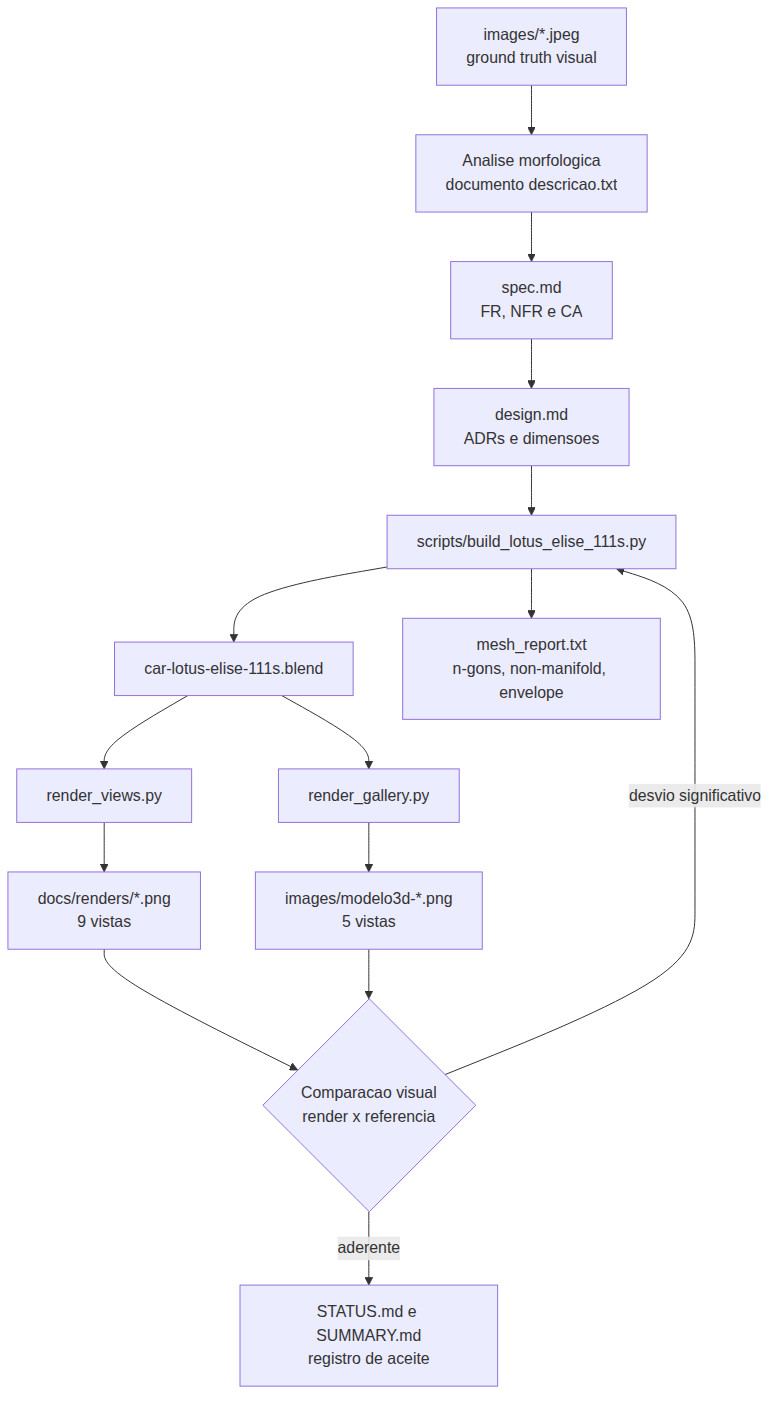
\includegraphics[width=\textwidth]{diagrams/pipeline-metodologico.png}
  \caption{Fluxo metodol\'ogico iterativo do trabalho. Os desvios identificados na compara\c{c}\~ao
           visual retornam ao script de constru\c{c}\~ao, e n\~ao a ajustes manuais na cena.}
  \label{fig:pipeline}
  \fonte{elaborado pelo autor (2026).}
\end{figure}

\section{Organiza\c{c}\~ao do trabalho}

Al\'em desta introdu\c{c}\~ao, o texto est\'a organizado em sete cap\'itulos. O
Cap\'itulo~\ref{ch:fundamentacao} apresenta a fundamenta\c{c}\~ao te\'orica: representa\c{c}\~ao de
superf\'icies, subdivis\~ao, sombreamento fisicamente baseado, pintura automotiva, motores de
render em tempo real e fundamentos de protocolos de contexto para agentes. O
Cap\'itulo~\ref{ch:relacionados} discute trabalhos relacionados em quatro frentes: modelagem
procedimental de ve\'iculos, pipelines de projeto assistido, engenharia reversa a partir de
fotografias e agentes que operam ferramentas externas. O Cap\'itulo~\ref{ch:metodos} descreve
materiais e m\'etodos, incluindo ambiente, arquitetura de \emph{software}, procedimento
experimental e amea\c{c}as \`a validade. O Cap\'itulo~\ref{ch:desenvolvimento} detalha a
implementa\c{c}\~ao. O Cap\'itulo~\ref{ch:resultados} apresenta os resultados quantitativos e a
an\'alise visual comparativa. O Cap\'itulo~\ref{ch:discussao} interpreta os resultados, discute
limita\c{c}\~oes e implicações. O Cap\'itulo~\ref{ch:conclusao} conclui e indica trabalhos
futuros. Os ap\^endices re\'unem a tabela de esta\c{c}\~oes do casco, a lista de materiais, a
lista de objetos da cena e a refer\^encia aos scripts.
